% =====================================================================
%  Shared sections (model, stability, control, swing-up) used by build_full_report.py and build_phase_reports.py
%  (layout follows the senior reference report: title page, contents,
%   numbered sections, code listings, tabulation, conclusion, contributions)
% =====================================================================
\documentclass[12pt,a4paper]{article}
\usepackage[a4paper,margin=1in]{geometry}
\usepackage[T1]{fontenc}
\usepackage{lmodern}
\usepackage{amsmath,amssymb,bm}
\usepackage{graphicx,float,booktabs,array,multirow}
\usepackage{xcolor}
\usepackage{algorithm}
\usepackage{algpseudocode}
\usepackage{fancyhdr}
\usepackage{enumitem}
\usepackage{caption}
\usepackage[hidelinks]{hyperref}

\pagestyle{fancy}
\fancyhf{}
\renewcommand{\headrulewidth}{0.6pt}
\fancyfoot[C]{\thepage}
\setlength{\headheight}{14.5pt}
\setlength{\parskip}{4pt}
\setlength{\parindent}{0pt}
\newcommand{\Nm}{\,\mathrm{N\,m}}
\captionsetup{font=small}

\begin{document}

\begin{titlepage}
\centering
\vspace*{2cm}

\includegraphics[width=4.2cm]{figures/logo-000.jpg}\\[3cm]
{\Huge Systems Thinking Project}\\[0.5cm]
{\Large Acrobot}\\[0.25cm]
{\large Phase 5: Reinforcement-Learning Swing-Up}\\[2.2cm]
\begin{tabular}{cc}
\textbf{Author:} Bhargav & \textbf{Author:} Sreekar\\
ID: 2025102061 & ID: 2025102074\\[0.8cm]
\textbf{Author:} Kaushik & \textbf{Author:} Divijat\\
ID: 2025102071 & ID: 2025102040
\end{tabular}
\vfill
{\large November 11, 2026}
\end{titlepage}

\tableofcontents
\newpage

\section{Introduction}
% =====================================================================
\subsection{What is an Acrobot?}
An acrobot is a two-link pendulum that hangs from a fixed pivot. The first link (the ``shoulder'' link) is free to rotate about the pivot; the second link is joined to the end of the first at the ``elbow''. The only motor sits at the elbow, so the shoulder is \emph{passive}. It is the robot version of a gymnast on a high bar who can only swing the legs at the hips. Because there are two degrees of freedom but only one actuator, the acrobot is a standard example of an \emph{underactuated} system [1], [2].

\subsection{Model}
The configuration is described by two generalised coordinates: $q_1$, the angle of link~1 from the downward vertical, and $q_2$, the angle of link~2 relative to link~1. The full state contains the angles and their rates:
\[
\mathbf q=\begin{bmatrix}q_1\\q_2\end{bmatrix},\qquad
\mathbf x=\begin{bmatrix}q_1\\q_2\\\dot q_1\\\dot q_2\end{bmatrix}.
\]
\begin{figure}[H]
\centering
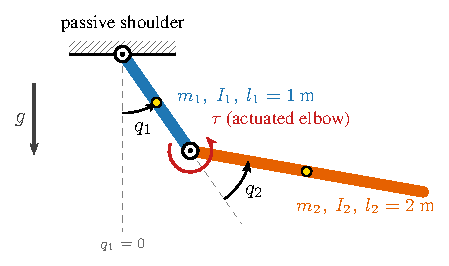
\includegraphics[width=0.42\textwidth]{figures/acrobot_diagram.pdf}
\caption{The acrobot: passive shoulder at the pivot, motor torque $\tau$ at the elbow; dots mark the centres of mass.}
\label{fig:acrobot}
\end{figure}

\subsection{Equations of Motion}
The dynamics (given in the Phase~1 helper and verified in Phase~1) are
\begin{equation}
M(q)\,\ddot q+C(q,\dot q)\,\dot q=\tau_g(q)+B\,\tau,\qquad B=\begin{bmatrix}0\\1\end{bmatrix},\qquad |\tau|\le 20\Nm .\label{eq:eom}
\end{equation}

\textbf{$\tau$ (Input Torque):} the torque of the elbow motor, the only quantity we command. $B=[0,\,1]^T$ says it acts on the elbow equation only.

\textbf{$M(q)$ (Inertia Matrix):} the resistance to angular acceleration. It depends on the elbow angle because the mass distribution changes as the arm folds:
\begin{equation}
M(q)=\begin{bmatrix}2.663+2\cos q_2 & 1.33+\cos q_2\\ 1.33+\cos q_2 & 1.33\end{bmatrix},\qquad \det M=1.7729-\cos^2q_2\ge0.7729>0 .
\end{equation}

\textbf{$C(q,\dot q)$ (Coriolis Matrix):} the coupling forces between the links (centrifugal and Coriolis effects):
\begin{equation}
C(q,\dot q)=\sin q_2\begin{bmatrix}-2\dot q_2 & -\dot q_2\\ \dot q_1 & 0\end{bmatrix}.
\end{equation}

\textbf{$\tau_g(q)$ (Gravity Torque):} the torque that gravity exerts on each joint, $\tau_g=-\partial U/\partial q$, with potential energy $U$:
\begin{equation}
U=-14.715\cos q_1-9.81\cos(q_1+q_2),\qquad
\tau_g(q)=-9.81\begin{bmatrix}1.5\sin q_1+\sin(q_1+q_2)\\ \sin(q_1+q_2)\end{bmatrix}.
\end{equation}

\textbf{System Parameters:}
\begin{gather*}
m_1=m_2=1\,\mathrm{kg},\qquad l_1=1\,\mathrm m,\qquad l_2=2\,\mathrm m,\qquad l_{c1}=0.5\,\mathrm m,\qquad l_{c2}=1\,\mathrm m,\\
I_1=0.083\,\mathrm{kg\,m^2},\qquad I_2=0.33\,\mathrm{kg\,m^2},\qquad g=9.81\,\mathrm{m\,s^{-2}}.
\end{gather*}

\subsection{Equilibria and Linear Model (from Phase 1)}
With $\tau^*=0$ the equilibria satisfy $\tau_g(q^*)=0$, i.e.\ $\sin q_1^*=0$ and $\sin(q_1^*+q_2^*)=0$. This gives four postures:
\begin{table}[H]
\centering
\caption{The four equilibria}
\begin{tabular}{|c|c|c|c|l|}
\hline
 & Posture & $(q_1^*,q_2^*)$ & $U$ [J] & Description\\ \hline
$E_1$ & down--down & $(0,0)$ & $-24.525$ & both links hanging\\
$E_2$ & down--up & $(0,\pi)$ & $-4.905$ & link 1 down, link 2 up\\
$E_3$ & up--up & $(\pi,0)$ & $+24.525$ & fully upright (target)\\
$E_4$ & up--down & $(\pi,\pi)$ & $+4.905$ & link 1 up, link 2 down\\ \hline
\end{tabular}
\end{table}
Linearizing about each equilibrium with $\tilde x=x-x^*$ gives
\begin{equation}
\dot{\tilde x}=A\tilde x+B_\ell\tilde\tau,\qquad A=\begin{bmatrix}0&I\\P&0\end{bmatrix},\qquad B_\ell=\begin{bmatrix}0\\r\end{bmatrix},\label{eq:lin}
\end{equation}
with $P=M(q^*)^{-1}K(q^*)$ and $r=M(q^*)^{-1}B$,
where $K=\partial\tau_g/\partial q$. The transfer functions from $\tau$ to the angles are
\begin{gather}
G_1(s)=\frac{r_1s^2+(P_{12}r_2-P_{22}r_1)}{\Delta(s)},\qquad
G_2(s)=\frac{r_2s^2+(P_{21}r_1-P_{11}r_2)}{\Delta(s)},\label{eq:tf}\\
\Delta(s)=s^4-\operatorname{tr}(P)\,s^2+\det P .\nonumber
\end{gather}
\begin{table}[H]
\centering
\caption{Transfer functions at the four equilibria (Phase 1)}
\label{tab:tf}
\small
\begin{tabular}{|c|l|l|l|}
\hline
 & $\Delta(s)$ & $N_1(s)$ ($\tau\to q_1$) & $N_2(s)$ ($\tau\to q_2$)\\ \hline
$E_1$ & $s^4+42.2410\,s^2+186.7719$ & $-3.0147\,(s^2+4.2103)$ & $6.0332\,(s^2+5.2595)$\\
$E_2$ & $s^4+8.4025\,s^2-186.7719$ & $-0.4270\,(s^2-29.7273)$ & $0.8578\,(s^2+7.3982)$\\
$E_3$ & $s^4-42.2410\,s^2+186.7719$ & $-3.0147\,(s^2-4.2103)$ & $6.0332\,(s^2-5.2595)$\\
$E_4$ & $s^4-8.4025\,s^2-186.7719$ & $-0.4270\,(s^2+29.7273)$ & $0.8578\,(s^2-7.3982)$\\ \hline
\end{tabular}
\end{table}

\subsection{Objective}
Replace the hand-designed Phase~4 swing-up with one learned by reinforcement learning, keep the same Phase~3 LQR for the final catch, and compare the two under $|\tau|\le20\Nm$: reliability, speed, control effort, and robustness when the real robot differs from the model.

Phase~4 provides the baseline: an energy-pumping swing-up with partial feedback linearization, gains $k=(20,2,3)$, which switches to the Phase~3 LQR ($Q=I$, $R=0.03$) when $\tilde x^TS\tilde x<5$.

% =====================================================================
% =====================================================================
\section{Reinforcement-Learning Swing-Up}
% =====================================================================
\subsection{Why Reinforcement Learning?}
The Phase~4 swing-up works, but it is built entirely from the model: the partial feedback linearization needs $M(q)$, $C(q,\dot q)$ and $\tau_g(q)$, and the energy target needs the exact masses and lengths. Reinforcement learning (RL) takes a different route. A neural-network policy learns \emph{by trial and error in a simulator} which torque to apply, guided only by a score (the reward). No equation of motion is written into the controller.
\begin{itemize}
\item \textbf{Question:} can a learned swing-up match or beat the hand-designed one under the same $20\Nm$ limit?
\item \textbf{Fair comparison:} both controllers hand over to the \emph{same} Phase~3 LQR inside the \emph{same} catch zone, so the only difference is who does the swing-up.
\item \textbf{Extra test:} what happens when the real robot differs from the model both controllers were designed or trained on?
\end{itemize}

\subsection{Hybrid Structure}
\begin{equation}
\tau=\begin{cases}\operatorname{sat}\big(-K\tilde x\big), & \tilde x^TS\tilde x<c_{sw}=5\quad\text{(catch: Phase 3 LQR, } R=0.03\text{)}\\[2pt] 20\,\pi_\theta(o),\ \ \pi_\theta(o)\in[-1,1], & \text{otherwise (learned swing-up, held for 20 ms)}\end{cases}
\end{equation}
RL only has to deliver the arm into the catch zone; it never has to learn to balance. The part we can prove (the LQR near the top) stays model-based, and the hard nonlinear part is learned. If the arm leaves the zone, control returns to the policy, the same retry logic as Phase~4.

\subsection{Environment}
The environment follows the Gymnasium interface and uses the given equations of motion~\eqref{eq:eom}, integrated with RK4.
\begin{table}[H]
\centering
\caption{RL environment}
\label{tab:env}
\resizebox{\textwidth}{!}{\begin{tabular}{|l|l|l|}
\hline
Element & Choice & Reason\\ \hline
Observation $o$ & $[\cos q_1,\ \sin q_1,\ \cos q_2,\ \sin q_2,\ \dot q_1/10,\ \dot q_2/10]$ & no jump at $\pm180^\circ$; inputs of order 1\\
Action $a$ & $a\in[-1,1]$, $\tau=20\,a$ & the torque limit is built in: the policy cannot exceed it\\
Control step & 20 ms (50 Hz), four RK4 steps of 5 ms & realistic control rate\\
Start & $|\tilde q_i(0)|\le0.6$ rad, $|\dot q_i(0)|\le0.5$ rad/s around hanging & same spread as the Phase 4 robustness test\\
Episode & 15 s; ends early on entering the catch zone & short episodes, one clear goal\\ \hline
\end{tabular}}
\end{table}

\subsection{Reward Design}
\begin{multline}
r=-\Big(\frac{E-E_{top}}{E_{top}}\Big)^2-0.3\,(1+\cos q_1)-0.1\,(1-\cos q_2)\\
-0.001\Big(\frac{\tau}{20}\Big)^2+100\cdot\mathbb 1[\text{enter catch zone}] .
\end{multline}
\begin{itemize}
\item \textbf{Energy term:} the same target as Phase~4. It tells the policy \emph{how much} energy to pump. Without it, RL tends to learn to spin the arm round and round, because a spinning arm passes near the top often.
\item \textbf{Angle terms:} $1+\cos q_1$ is 0 when link~1 points up; $1-\cos q_2$ is 0 when the elbow is straight. They tell the policy \emph{where} to go.
\item \textbf{Torque term:} a small penalty that discourages wasted effort and bang--bang control.
\item \textbf{Catch bonus:} $+100$ for reaching the region where the LQR takes over; the episode then ends.
\end{itemize}

\subsection{Algorithm: Soft Actor-Critic (SAC)}
SAC [8] learns a stochastic policy $\pi_\theta$ (the actor) and two action-value networks $Q_\phi$ (the critics) that maximize reward plus entropy:
\begin{equation}
J(\pi)=\mathbb E\Big[\sum_t\gamma^t\big(r_t+\alpha\,\mathcal H(\pi(\cdot\mid o_t))\big)\Big].
\end{equation}
The entropy term $\mathcal H$ keeps the policy exploring, and $\alpha$ is tuned automatically. SAC suits this problem because the torque is continuous and SAC reuses past experience (off-policy), so it needs relatively few simulated swings.
\begin{table}[H]
\centering
\caption{Training settings (stable-baselines3 [9])}
\resizebox{\textwidth}{!}{\begin{tabular}{|l|l|}
\hline
Setting & Value\\ \hline
Networks & 2 hidden layers $\times$ 256 units (actor and critics)\\
Discount $\gamma$, learning rate, batch & $0.99$, $3\times10^{-4}$, 256\\
Replay buffer & 300\,000 transitions\\
Parallel environments, seed & 4, 0\\
Training length & $10^6$ steps $=$ 9\,206 episodes, 12.4 min on a laptop CPU\\ \hline
\end{tabular}}
\end{table}

\subsection{Training}
\begin{figure}[H]
\centering
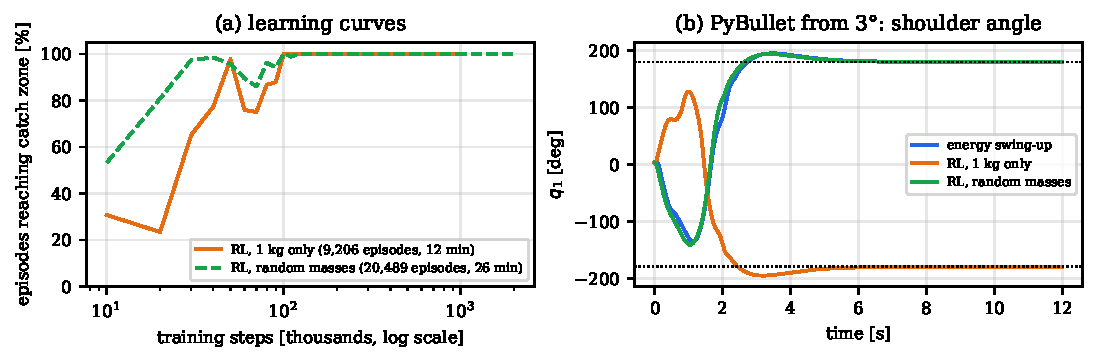
\includegraphics[width=\textwidth]{figures/fig_training.pdf}
\caption{(a) Share of training episodes that reached the catch zone, for the original policy and for the robust policy of Section~\ref{sec:robust} (log scale). (b) PyBullet runs from $3^\circ$: the original RL policy swings the other way and ends at $q_1=-180^\circ$, the same upright pose as $+180^\circ$; the robust policy swings the same way as the energy law.}
\label{fig:training}
\end{figure}
\textbf{Observations:}
\begin{itemize}
\item The policy first reached the catch zone in every episode after about $10^5$ steps (72~s of training) and stayed at 100\% for the remaining $9\times10^5$ steps.
\item Episodes kept getting shorter (more episodes per $10^4$ steps: 54 at $10^5$, 110 at $10^6$): the policy kept learning to reach the top faster.
\item The robust policy (Section~\ref{sec:robust}), which faces a different robot in every episode, also first reached 100\% after about $10^5$ steps. Over its remaining $1.9\times10^6$ steps it never dropped below 98.8\%.
\end{itemize}

\subsection{Results: Correct Model}
Both controllers were tested from the same 40 random starts as Phase~4. A start counts as held if it is caught and balanced within 30~s. (This is why the energy controller scores 35 rather than the Phase~4 value of 39, which allowed 40~s.)
\begin{table}[H]
\centering
\caption{RL vs.\ energy swing-up, correct masses ($|\tau|\le20\Nm$)}
\label{tab:rlnom}
\begin{tabular}{|l|c|c|}
\hline
Metric & Energy swing-up & RL swing-up (SAC)\\ \hline
Held (of 40) & 35 & \textbf{40}\\
Median time to first catch & 3.98 s & \textbf{1.71 s}\\
Time at the torque limit & 8.8\% & \textbf{0.1\%}\\
Median elbow work & 244.9 J & \textbf{144.5 J}\\
PyBullet from $3^\circ$: first catch & 2.17 s & \textbf{1.76 s}\\ \hline
\end{tabular}
\end{table}
\textbf{Observations:}
\begin{itemize}
\item \textbf{Reliability:} RL caught all 40 starts; the energy law caught 35 within 30~s.
\item \textbf{Speed:} RL reaches the top more than twice as fast (median 1.71 s vs.\ 3.98 s).
\item \textbf{Control effort:} RL almost never saturates the motor (0.1\% vs.\ 8.8\%) and uses 41\% less work. In Phase~4 saturation was what broke the energy law; the policy learned a timing that stays within $20\Nm$ by itself.
\end{itemize}

\subsection{Results: Wrong Model}
The real robot never matches the model exactly. The same 40 starts were rerun with both link masses changed by $\pm20\%$ (inertias scaled with them). Both controllers still assume 1~kg links.
\begin{table}[H]
\centering
\caption{Robustness to the link masses (held of 40, within 30 s)}
\label{tab:rlrob}
\begin{tabular}{|l|c|c|}
\hline
Link masses & Energy swing-up & RL swing-up (SAC)\\ \hline
$-20\%$ (0.8 kg) & 37 & 38\\
correct (1.0 kg) & 35 & 40\\
$+20\%$ (1.2 kg) & \textbf{35} & \textbf{15}\\ \hline
\end{tabular}
\end{table}
\begin{itemize}
\item \textbf{The energy law degrades gracefully} (35--37 of 40 in every case). It is built from physics: it pumps until $E=E_{top}$, so a heavier arm just takes a little longer (median 5.4~s instead of 4.0~s).
\item \textbf{RL collapses on heavier links} (15 of 40). It practised only on 1~kg links, so it learned the \emph{timing of that particular robot}, not the physics. It still reaches the catch zone in all 40 runs, but in a state from which the LQR cannot hold the heavier arm; it then repeats nearly the same approach (a median of 13 hand-overs in 30~s instead of 2).
\item \textbf{The fix} is to let the policy practise on many different robots (Section~\ref{sec:robust}).
\end{itemize}

\subsection{Making the Policy Robust}\label{sec:robust}
A second policy was trained with exactly \textbf{two changes}. Everything else (network, reward, catch zone, LQR and SAC settings) is the same, so any difference in the results comes from these two changes.
\begin{table}[H]
\centering
\caption{The two changes for the robust policy}
\label{tab:robustchanges}
\small
\begin{tabular}{|>{\raggedright\arraybackslash}p{2.5cm}|>{\raggedright\arraybackslash}p{3.0cm}|>{\raggedright\arraybackslash}p{4.6cm}|>{\raggedright\arraybackslash}p{4.0cm}|}
\hline
& \textbf{Original policy} & \textbf{Robust policy} & \textbf{Why}\\ \hline
1. Link masses in training & always 1 kg & new random $m_1,m_2\in[0.7,1.3]$ kg in every episode & it cannot memorise one robot's timing\\ \hline
2. Observation & the 6 numbers of Table~\ref{tab:env} & the same 6, plus the missing energy $(E_{top}-E)/E_{top}$ & the quantity the energy law steers by\\ \hline
Training length & $10^6$ steps, 9\,206 episodes, 12.4 min & $2\times10^6$ steps, 20\,489 episodes, 25.9 min & many robots make a harder task\\ \hline
\end{tabular}
\end{table}
The extra input is computed from the other six with the nominal 1~kg model, exactly as the energy controller computes it. It therefore adds no new information: it is a hint that makes the important quantity explicit. Change~1 is the real fix (this is called \emph{domain randomization}). By the end of training the robust policy reached the catch zone in 100\% of episodes, as the original did.

All three swing-ups were then tested from the same 40 starts with five link masses. Two of them (0.6 and 1.4 kg) lie \emph{outside} the range the robust policy practised on. Every controller still assumes 1~kg links.
\begin{table}[H]
\centering
\caption{Held of 40 random starts (within 30 s) for five link masses}
\label{tab:rlrob2}
\resizebox{\textwidth}{!}{\begin{tabular}{|l|c|c|c|}
\hline
True link masses & Energy swing-up & RL, 1 kg only & RL, random masses\\ \hline
0.6 kg ($-40\%$, never practised) & 39 & 2 & \textbf{40}\\
0.8 kg ($-20\%$) & 37 & 38 & \textbf{40}\\
1.0 kg (correct) & 35 & \textbf{40} & \textbf{40}\\
1.2 kg ($+20\%$) & 35 & 15 & \textbf{40}\\
1.4 kg ($+40\%$, never practised) & \textbf{33} & 3 & 2\\ \hline
\end{tabular}}
\end{table}
\begin{figure}[H]
\centering
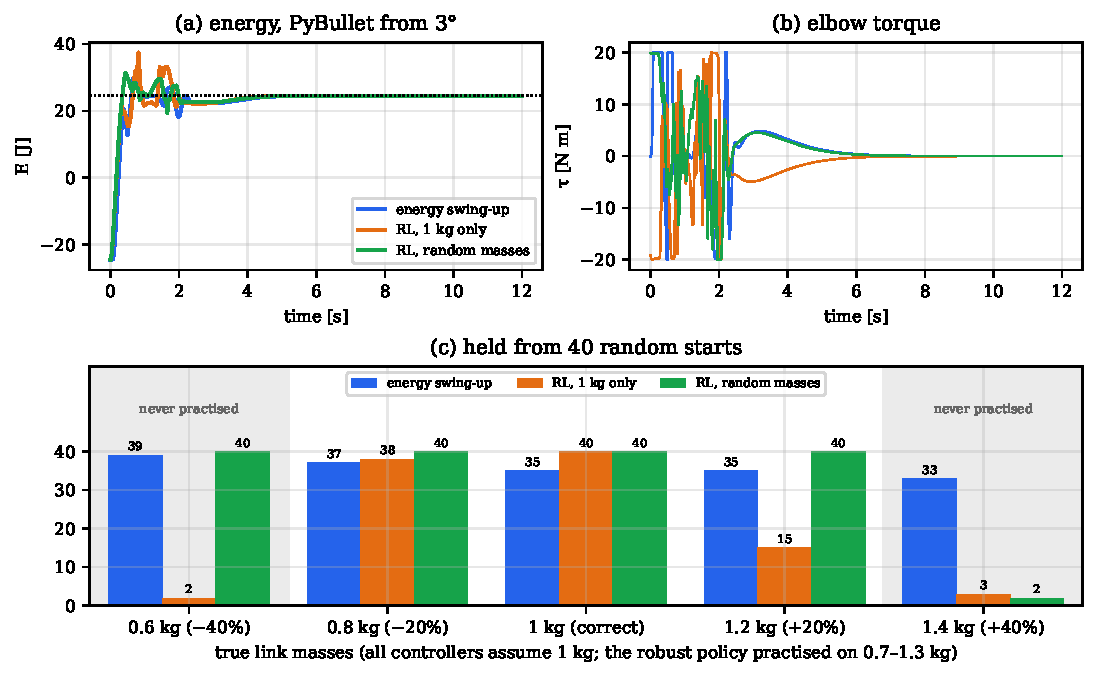
\includegraphics[width=\textwidth]{figures/fig_compare.pdf}
\caption{(a) Energy and (b) elbow torque in PyBullet from $3^\circ$ for the three swing-ups; (c) starts held for five link masses. Shaded: masses the robust policy never practised on.}
\label{fig:compare}
\end{figure}
\textbf{Observations:}
\begin{itemize}
\item \textbf{Inside the practised range the problem is solved:} 40 of 40 at every mass from 0.8 to 1.2~kg. At $+20\%$ the score rises from 15 to 40.
\item \textbf{No price on the correct model:} the robust policy also holds 40 of 40, with the same median catch time (1.71~s), no saturation (0.0\%) and 10\% less elbow work (130.0~J vs.\ 144.5~J). In PyBullet from $3^\circ$ it catches at 1.89~s (original 1.76~s).
\item \textbf{Lighter than ever practised (0.6~kg):} still 40 of 40. The original policy managed only 2, and in 25 of its 40 runs it never even reached the catch zone.
\item \textbf{Much heavier than ever practised (1.4~kg):} only 2 of 40, while the energy law still holds 33. The policy reaches the catch zone in all 40 runs, but the hand-over fails again and again (a median of 12 hand-overs in 30~s, against 1 for the energy law). The energy law also loses many first catches, but each new approach is different, so a later catch usually works; the policy repeats nearly the same approach.
\item \textbf{Why the hand-over is the weak point:} the reward ends the episode as soon as the arm \emph{enters} the catch zone. The policy is never told whether the LQR then holds the arm, so it never learned to deliver the arm in an easy-to-catch state.
\end{itemize}
\textbf{Lesson:} a learned controller is reliable over the variety of robots it practised on (here, also somewhat beyond it on the light side). A physics-based law knows \emph{why} it works, so it extrapolates further. Two natural next steps would be to reward holding rather than only arriving (end each episode only after the LQR has held the arm for, say, 1~s) and to widen the mass range.

\subsection{Discussion}
\begin{enumerate}
\item \textbf{Why RL is faster and gentler.} The energy law fixes the elbow motion through $v$ and pays for it with saturation. The policy is free to choose any torque profile and is rewarded for reaching the top quickly with little effort, so it found a timing that pumps energy faster without hitting the limit.
\item \textbf{Why RL was fragile, and what fixed it.} Its knowledge is implicit in $256\times256$ hidden units fitted to the robots it practised on. Practising on one robot gave that robot's timing; practising on many made it robust over that range. Nothing in it says ``pump until $E=E_{top}$'', however, so far outside that range (1.4~kg) it can still fail where the energy law does not.
\item \textbf{Guarantees.} The LQR catch has a Lyapunov certificate (Phase~3). The learned part has none: its performance is known only from tests, which is why it was tested on 40 starts, in a second simulator (PyBullet) and with five different link masses.
\item \textbf{Hybrid design.} Learning the hard nonlinear part and keeping the provable part near the top gave the best of both: the speed of RL, and a guaranteed final balance.
\end{enumerate}
% =====================================================================
\section{Simulations and Code}
% =====================================================================
\subsection{Training and Evaluation Pipeline}
The work is in \texttt{phase5\_rl/}; \texttt{bash run\_pipeline.sh 1000000} runs every step in order (about 50 minutes on a laptop CPU):
\begin{enumerate}
\item \textbf{Model check:} the mass-parametric model reproduces the given equations of motion to $10^{-13}$.
\item \textbf{Training} (\texttt{train.py}): SAC for $10^6$ steps on 1~kg links, then the robust policy (option \texttt{-{}-robust}) for $2\times10^6$ steps. Both policies are saved in the folder \texttt{policies/}, each with its learning curve.
\item \textbf{Evaluation} (\texttt{evaluate.py}): all three swing-ups from 40 random starts with five link masses (0.6--1.4~kg), plus PyBullet runs; writes \texttt{results.json} and the figures above.
\item \textbf{Video} (\texttt{manim-sim/rl\_vs\_energy.py}): the explanatory comparison animation.
\end{enumerate}
Libraries: Gymnasium 1.4 (environment interface), stable-baselines3 2.9 (SAC), PyTorch 2.15, PyBullet.

\subsection{Python Codes}
The files are listed below; the algorithms they implement follow as pseudo-code.
\begin{table}[H]
\centering
\caption{Python files (\texttt{phase5\_rl/})}
\resizebox{\textwidth}{!}{\begin{tabular}{|l|l|}
\hline
File & Purpose\\ \hline
\texttt{acrobot\_env.py} & Gymnasium environment, mass-parametric model, reward, RL $\to$ LQR controller\\
\texttt{train.py} & SAC training; saves the policy and the learning curve\\
\texttt{evaluate.py} & 40-start and wrong-mass tests, PyBullet runs, figures\\
\texttt{run\_pipeline.sh} & runs model check, training, evaluation and video in order\\ \hline
\end{tabular}}
\end{table}

\begin{algorithm}[H]
\caption{Learned swing-up: environment step and SAC training (\texttt{acrobot\_env.py}, \texttt{train.py})}
\label{alg:p5train}
\begin{algorithmic}[1]
\Function{Reset}{}
  \State $x\gets$ random start near hanging; \quad $m_1,m_2\gets1$ kg \Comment{robust policy: $m_i\sim U[0.7,1.3]$ kg}
\EndFunction
\Function{EnvStep}{$x$, action $a\in[-1,1]$}
  \State $\tau\gets20a$; \quad integrate the model with masses $m_1,m_2$ for 20 ms (four RK4 steps of 5 ms)
  \State $r\gets-((E-E_{top})/E_{top})^2-0.3(1+\cos q_1)-0.1(1-\cos q_2)-0.001(\tau/20)^2$
  \If{$\tilde x^TS\tilde x<5$} \State $r\gets r+100$; episode ends \Comment{reached the LQR catch zone}
  \EndIf
  \State $o\gets[\cos q_1,\sin q_1,\cos q_2,\sin q_2,\dot q_1/10,\dot q_2/10]$ \Comment{robust policy: append $(E_{top}-E)/E_{top}$}
  \State \Return $o$, $r$
\EndFunction
\State initialise actor $\pi_\theta$, critics $Q_{\phi_1},Q_{\phi_2}$ (2$\times$256 each), empty replay buffer
\For{$10^6$ environment steps (4 environments in parallel)}
  \State $a\sim\pi_\theta(\cdot\mid o)$; \quad $(o',r)\gets$ \Call{EnvStep}{$x,a$}; \quad store $(o,a,r,o')$ in the buffer
  \State sample a batch of 256; update the critics towards $r+\gamma(\min_iQ_{\phi_i}(o',a')-\alpha\log\pi_\theta(a'\mid o'))$
  \State update the actor to maximise $\min_iQ_{\phi_i}(o,a)-\alpha\log\pi_\theta(a\mid o)$; tune $\alpha$
\EndFor
\State save $\pi_\theta$
\end{algorithmic}
\end{algorithm}
\begin{algorithm}[H]
\caption{Learned swing-up: RL $\to$ LQR controller and evaluation (\texttt{acrobot\_env.py}, \texttt{evaluate.py})}
\label{alg:p5eval}
\begin{algorithmic}[1]
\Function{RLController}{$x$}
  \If{$\tilde x^TS\tilde x<5$} \State \Return $\operatorname{sat}(-K\tilde x)$ \Comment{same upright LQR catch}
  \EndIf
  \State every 20 ms: $\tau\gets20\,\pi_\theta(o)$ (deterministic); hold it in between
  \State \Return $\tau$
\EndFunction
\For{link masses $\in\{0.6,\ 0.8,\ 1.0,\ 1.2,\ 1.4\}$ kg} \Comment{controllers always assume 1 kg}
  \For{each of the 40 random starts, for the energy and both RL controllers}
    \State simulate 30 s; record held, first catch time, torque saturation, elbow work and hand-overs
  \EndFor
\EndFor
\end{algorithmic}
\end{algorithm}


\subsection{Animation}
A 2K Manim animation comparing the RL and energy swing-ups is in \url{phase5_rl/RL_vs_Energy_SwingUp_2K.mp4}.

% =====================================================================
\section{Tabulation}
% =====================================================================
\begin{table}[H]
\centering
\caption{Energy swing-up vs.\ the two RL swing-ups: summary (40 random starts, held within 30 s)}
\resizebox{\textwidth}{!}{\begin{tabular}{|l|c|c|c|}
\hline
Criterion & Energy swing-up & RL, 1 kg only & RL, random masses\\ \hline
Held, correct masses & 35/40 & 40/40 & 40/40\\
Median time to catch & 3.98 s & 1.71 s & 1.71 s\\
Time at the torque limit & 8.8\% & 0.1\% & 0.0\%\\
Median elbow work & 244.9 J & 144.5 J & 130.0 J\\
Held, masses $-40\%$ (never practised) & 39/40 & 2/40 & 40/40\\
Held, masses $-20\%$ & 37/40 & 38/40 & 40/40\\
Held, masses $+20\%$ & 35/40 & 15/40 & 40/40\\
Held, masses $+40\%$ (never practised) & 33/40 & 3/40 & 2/40\\
Needs the equations of motion & yes & no (only a simulator) & no (only a simulator)\\
Explainable / provable & yes (energy argument) & no (tested only) & no (tested only)\\
Design effort & 3 gains + search & reward design + 12 min training & same + 26 min training\\ \hline
\end{tabular}}
\end{table}

% =====================================================================
\section{Conclusion}
% =====================================================================
A swing-up policy learned with Soft Actor-Critic, handing over to the same Phase~3 LQR, outperformed the hand-designed energy swing-up on the model it was trained on. It held 40 of 40 random starts instead of 35, reached the top more than twice as fast (1.7~s vs.\ 4.0~s), almost never saturated the motor, and used 41\% less work. It learned this in 12 minutes from a reward alone, with no equations of motion in the controller.

The first policy paid for this with robustness. With links 20\% heavier than in training it held only 15 of 40 starts, while the physics-based law still held 35, because the policy had learned one robot's timing rather than the energy principle. A second policy, trained with only two changes (random link masses between 0.7 and 1.3~kg in every episode, and the missing energy as one extra input), held 40 of 40 at every mass from 0.6 to 1.2~kg at no cost on the correct model. At 1.4~kg, far heavier than anything it practised on, it still failed (2 of 40) where the energy law held 33: a learned controller is reliable over the variety it practised on, while a physics-based law extrapolates further. The hybrid design (learn the hard nonlinear swing-up, keep the provable LQR catch) gives the speed of learning with a guaranteed final balance.

% =====================================================================
\section{Contributions}
% =====================================================================
% Fill in who did what before submitting.
\begin{enumerate}
\item Report compilation -- \underline{\hspace{4cm}}
\item RL problem and environment design (Sections 2.1--2.4) -- \underline{\hspace{4cm}}
\item SAC training (Sections 2.5--2.6) -- \underline{\hspace{4cm}}
\item Results and robust policy (Sections 2.7--2.9) -- \underline{\hspace{4cm}}
\item Discussion (Section 2.10) -- \underline{\hspace{4cm}}
\item Python code and figures -- \underline{\hspace{4cm}}
\item Animation (Manim) -- \underline{\hspace{4cm}}
\end{enumerate}

\begin{thebibliography}{9}
\bibitem{spong} M.~W. Spong, ``The swing up control problem for the Acrobot,'' \emph{IEEE Control Systems Magazine}, vol.~15, no.~1, pp.~49--55, 1995.
\bibitem{tedrake} R.~Tedrake, \emph{Underactuated Robotics}, MIT, 2024. Available: https://underactuated.csail.mit.edu
\bibitem{skogestad} S.~Skogestad and I.~Postlethwaite, \emph{Multivariable Feedback Control}, 2nd ed., Wiley, 2005.
\bibitem{khalil} H.~K. Khalil, \emph{Nonlinear Systems}, 3rd ed., Prentice Hall, 2002.
\bibitem{pybullet} E.~Coumans and Y.~Bai, ``PyBullet, a Python module for physics simulation,'' 2016--2024. Available: https://pybullet.org
\bibitem{youla} D.~C. Youla, J.~J. Bongiorno and C.~N. Lu, ``Single-loop feedback-stabilization of linear multivariable dynamical plants,'' \emph{Automatica}, vol.~10, pp.~159--173, 1974.
\bibitem{anderson} B.~D.~O. Anderson and J.~B. Moore, \emph{Optimal Control: Linear Quadratic Methods}, Prentice Hall, 1990.
\bibitem{sac} T.~Haarnoja, A.~Zhou, P.~Abbeel and S.~Levine, ``Soft actor-critic: Off-policy maximum entropy deep reinforcement learning with a stochastic actor,'' in \emph{Proc. ICML}, 2018.
\bibitem{sb3} A.~Raffin, A.~Hill, A.~Gleave, A.~Kanervisto, M.~Ernestus and N.~Dormann, ``Stable-Baselines3: Reliable reinforcement learning implementations,'' \emph{JMLR}, vol.~22, no.~268, pp.~1--8, 2021.
\end{thebibliography}

\end{document}
